\documentclass[]{article}
\usepackage{geometry}
\geometry{
a4paper,
total={170mm,257mm},
left=20mm,
top=20mm,
}
\usepackage{booktabs} 
\usepackage{longtable}
\usepackage{appendix}
\usepackage{graphicx}
\usepackage{subcaption}
\usepackage{listings}
\usepackage[justification=centering]{caption}
\usepackage{hyperref}
\usepackage{enumitem}
\usepackage[utf8]{inputenc}
\usepackage{float}
\usepackage[autostyle]{csquotes} 
\DeclareTextFontCommand{\helvetica}{\fontfamily{phv}\selectfont}
\setlength{\parindent}{4em}
\setlength{\parskip}{1em}
\linespread{1.5}

\usepackage[table]{xcolor}
\usepackage{graphicx}
\usepackage{adjustbox}

\title{PAC3 Desenvolupament del treball - Fase 2}
\date{20 de Maig 2019}
\author{Vasyl Druchkiv \\ Estudiant del Màster de Bioestadística i Bioinformàtica}
\renewcommand{\contentsname}{Índice}
\usepackage{setspace}


\renewcommand\paragraph{\@startsection{paragraph}{4}{\z@}%
{-2.5ex\@plus -1ex \@minus -.25ex}%
{1.25ex \@plus .25ex}%
{\normalfont\normalsize\bfseries}}

\begin{document}
\maketitle
\makeatletter

\makeatother
\begin{spacing}{0.1}
\tableofcontents
\end{spacing}

\begin{center}
\noindent\rule{8cm}{0.4pt}
\end{center}

\section{Descripció de l'avenç del projecte} 
El comentari del professor després de la primera PAC incloïa els punts següents:

\begin{itemize}
\item Pensar en la memòria on he d'explicar els mètodes que utilitzo;

\item Pensar en el manual i les ajudes del programa. Es fonamental que sigui el més autoexplicatiu possible;

\item Preparar un instal·lador de forma que no calgui entrar en el codi. De fet alguns paquets no s'instal•len com els altres i això fa que l'execució de l'app no sigui immediata.

\end{itemize}

Els punts són importants i van definir el full de ruta de la PAC actual. Explico punt per punt el que he pogut fer per realitzar quests punts.

\subsection{Instal·lació de l'aplicació}

La solució més plausible i ràpida era empaquetar tota l'aplicació dins d'un paquet R i fer-la disponible d'aquesta manera en el GitHub. Hi havia també dues opcions més: 

\begin{itemize}
\item Publicar l'aplicació a CRAN
\item Publicar l'aplicació en un servidor Shiny
\end{itemize}
La primera opció, la publicació en CRAN, no l’he contemplat encara, perquè la solució no és immediata, sino és un procès que no és fàcil i pot tardar fins que el paquet estigui publicat amb èxit. Com comenta \cite{HWick} \enquote{submitting to CRAN is a lot more work than just providing a version on github, but the vast majority of R users do not install packages from github, because CRAN provides discoverability, ease of installation and a stamp of authenticity. The CRAN submission process can be frustrating, but it’s worthwhile...}. Normalment els paquets han d’estar en perfectes condicions abans d'entregar-los i seran revisats manualmet per un equip de voluntaris. D'aquesta manera l'aplicació no seria avaluable dins del marc temporal previst per al treball de màster. A més a més considero que podria millorar encara més l'aplicació abans d'entregar-lo.

La segona opció, la publicació via Shiny Server, és molt interessant, però implicaria un treball considerable per configurar el servidor. Com que ho faria per primera vegada, no puc assegurar que tot estaria preparat a temps. A més a més encara tinc pendents la redacció del manual (que explicaré més endavant) i de la memòria. 

Per tant, el paquet \helvetica{PathwayApp} es pot instal•lar des del repositori GitHub seguint els passos següents:

\begin{enumerate}
\item Instal·lar, si encara no està fet, la versió actual de R;

\item Instal·lar, si encara no està fet, el Bioconductor;

\item Instal·lar, si encara no està fet, el paquet \helvetica{devtools}

\begin{lstlisting}[language=R]
install.packages(``devtools'')
library(devtools)
\end{lstlisting}

\item Instal·lar el paquet \helvetica{PathwayApp}

\begin{lstlisting}[language=R]
devtools::install_github("vdruchkiv/TFM/5_Packages/PathwayApp/PathwayApp")
\end{lstlisting}

\item Iniciar l'aplicació 
\begin{lstlisting}[language=R]
PathwayApp::runPathwayApp()
\end{lstlisting}
\end{enumerate}

La funció \helvetica{runPathwayApp()} iniciarà la comprovació dels paquets necessaris i començarà l'aplicació. Els paquets següents seran instal·lats, si no ho són encara:

\begin{center}
\begin{tabular}{||c | c ||} 
\hline\hline 
\textbf{Paquet} & \textbf{Font} \\ [0.5ex] 
\hline\hline
clusterProfiler & Bioconductor \\
\hline
ReactomePA & Bioconductor \\
\hline
pathview & Bioconductor \\ 
\hline
pathviewPatched & GitHub vdruchkiv/TFM\\
\hline
dplyr & CRAN \\
\hline 
ggplot2 & CRAN \\
\hline
knitr & CRAN \\
\hline
kableExtra & CRAN \\
\hline
formattable & CRAN \\
\hline
shiny & CRAN \\
\hline 
shinydashboard & CRAN \\ 
\hline
shinyhelper & CRAN \\
\hline 
shinycssloaders & CRAN\\
\hline\hline
\end{tabular}
\end{center}

\subsection{Manual i les ajudes del programa}

Per facilitar l'ús de l’aplicació he pensat com es podria fer de manera més intuïtiva possible. Primer cal destacar que com a llengua de manual he elegit l’anglès per poder fer l'ús de l'aplicació el més inclusiu possible. Segon, l'usuari pot accedir tant al manual com a l'ajuda, que es guarden en arxius .Md separats. Per accedir al manual l'usuari ha de clicar al símbol d’interrogació a prop del títol \textbf{Pathway analysis}:
\begin{figure}[H]
\centering
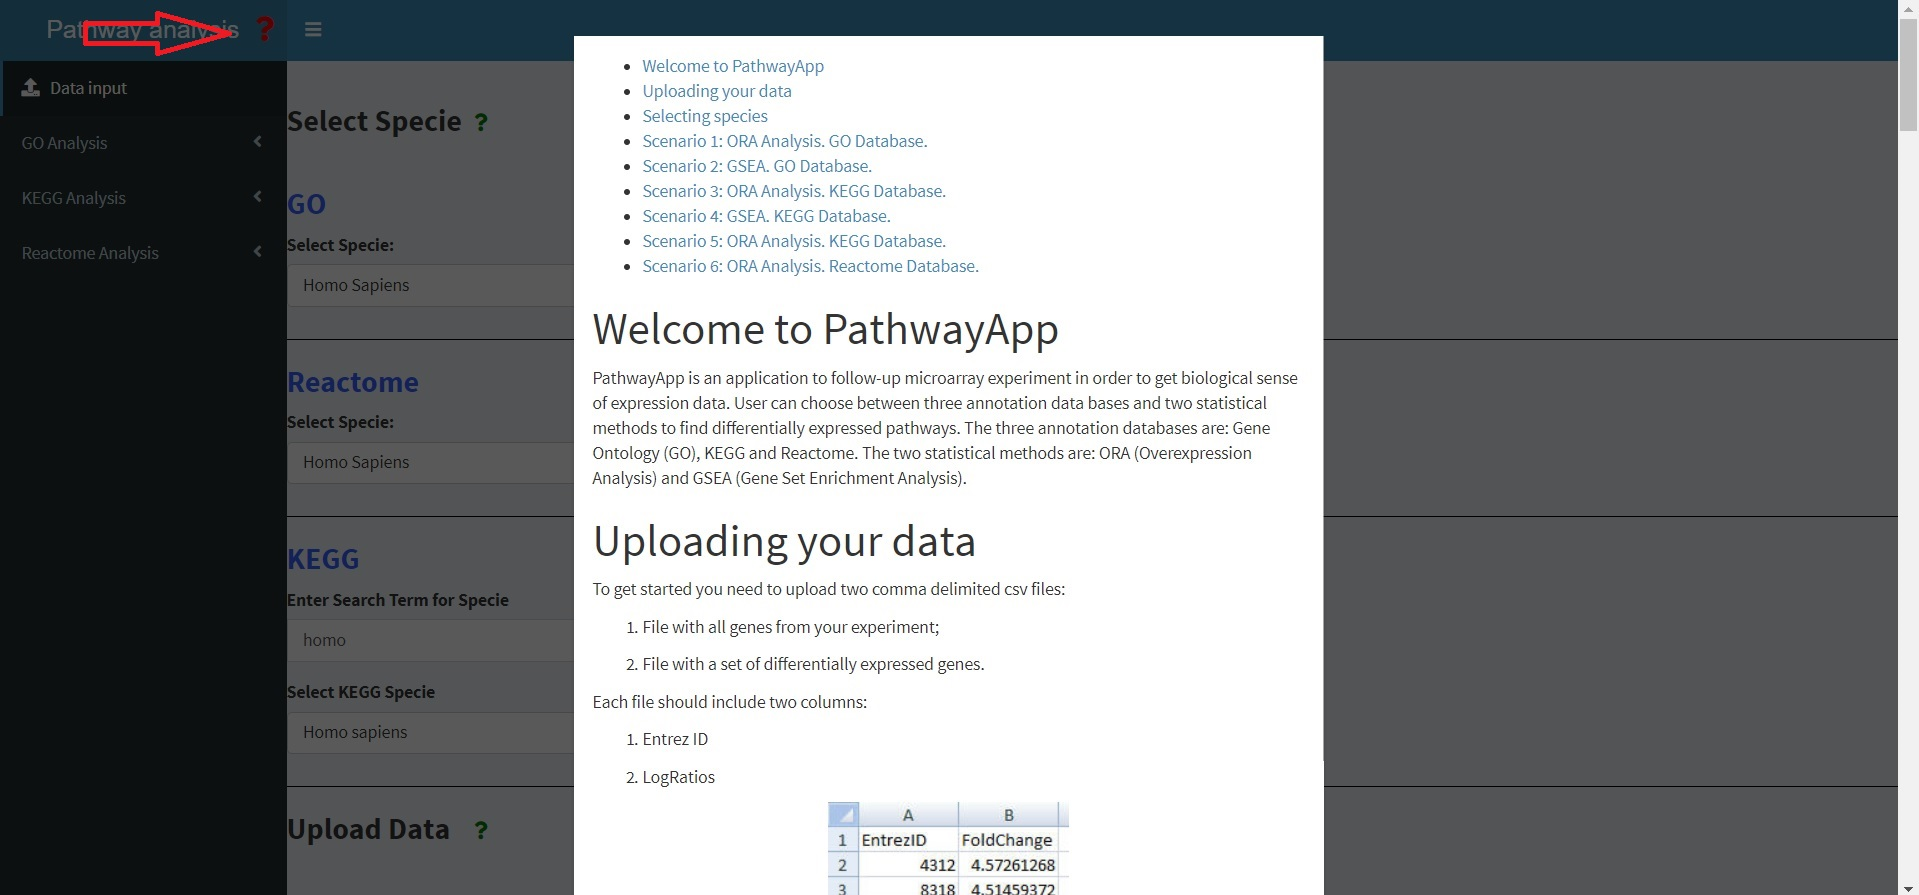
\includegraphics[width=1\textwidth]{Manual.jpg} 
\caption{Manual per a aplicació}
\end{figure}

Com es veu hi ha apartats diferents. Depenent dels objectius de l'usuari, aquest pot seleccionar l'apartat que més l'interessi. Així, si l'usuari vol fer l'anàlisi ORA amb l'anotació KEGG pot navegar en la secció |textbf{Scenario 3: ORA Analysis. KEGG Database}. 

\begin{figure}[H]
\centering
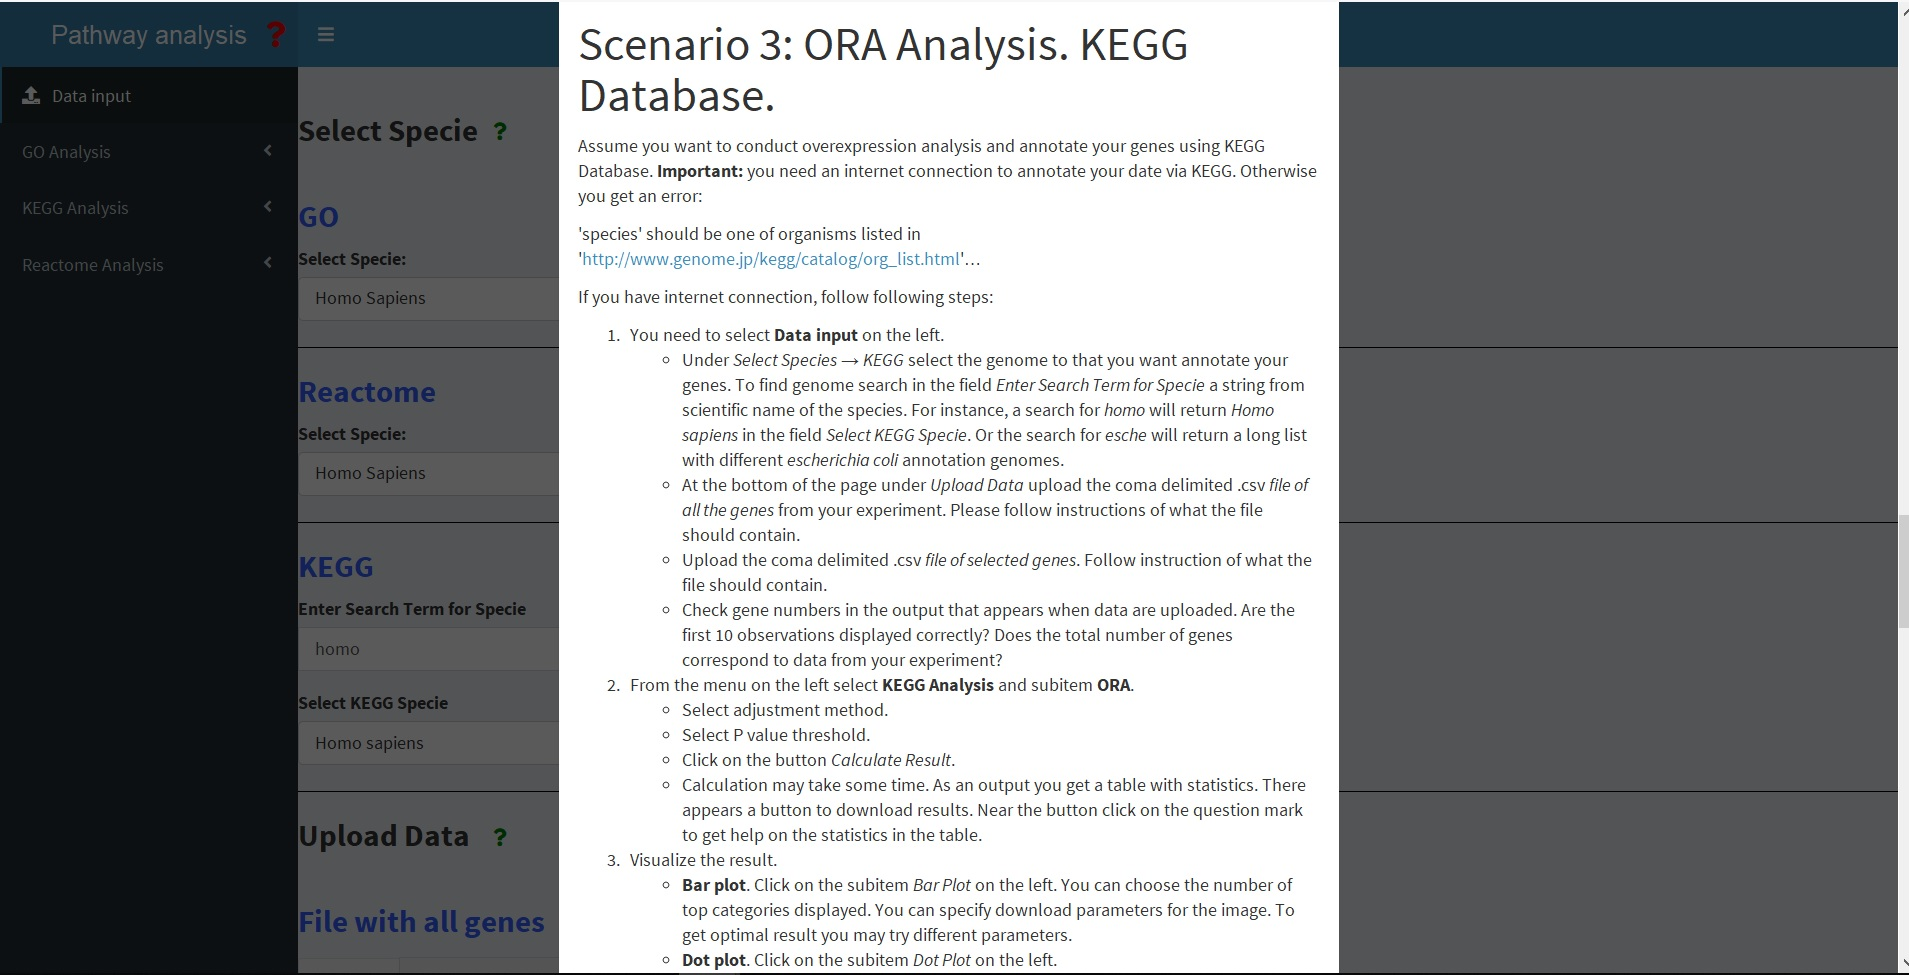
\includegraphics[width=1\textwidth]{Manual2.jpg} 
\caption{Manual per a l'anàlisi ORA amb l'anotació KEGG}
\end{figure}


També, l'usuari pot accedir a l'ajuda clicant als símbols d'interrogació distribuïts per l’aplicació en els llocs que penso que poden generar dubtes. 

Per fer-ho possible s'utilitza el paquet \helvetica{shinyhelper} que s'instal·la en executar la funció \helvetica{runPathwayApp()}.

\begin{figure}[H]
\centering
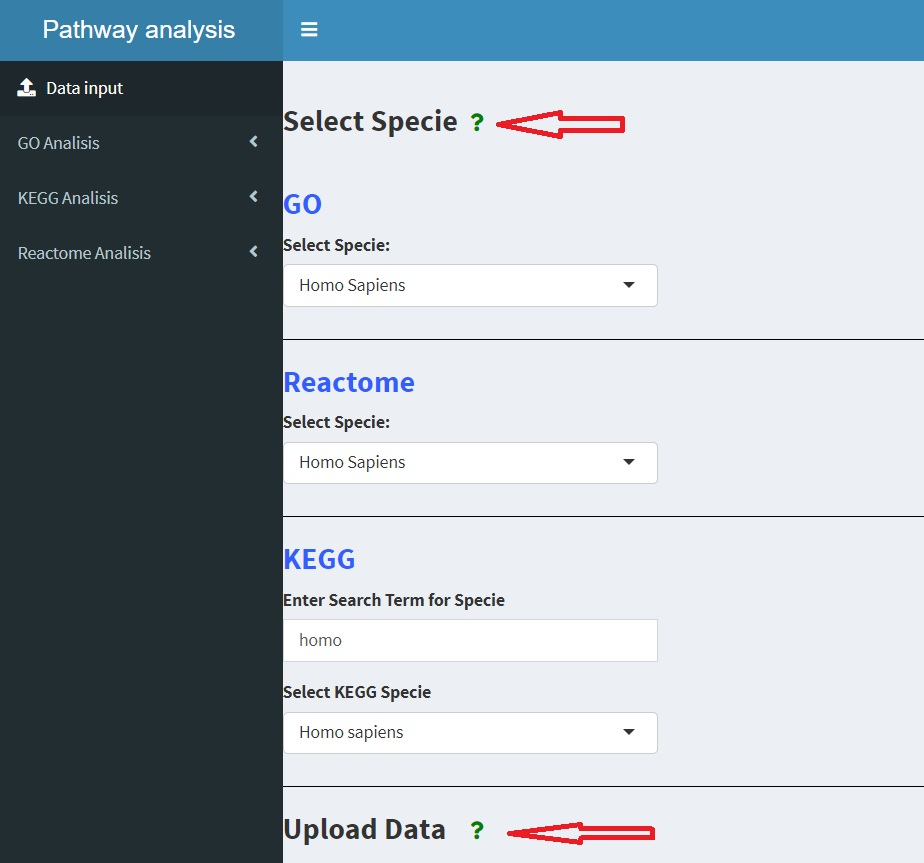
\includegraphics[width=0.7\textwidth]{Help_Data_Input.jpg} 
\caption{Senyals d'ajuda}
\end{figure}

El clic en aquests senyals fa que aparegui una finestreta amb la informació d'ajuda.

Aquí hi ha informació de l'apartat \textbf{Data Input}:

\begin{figure}[H]
\centering
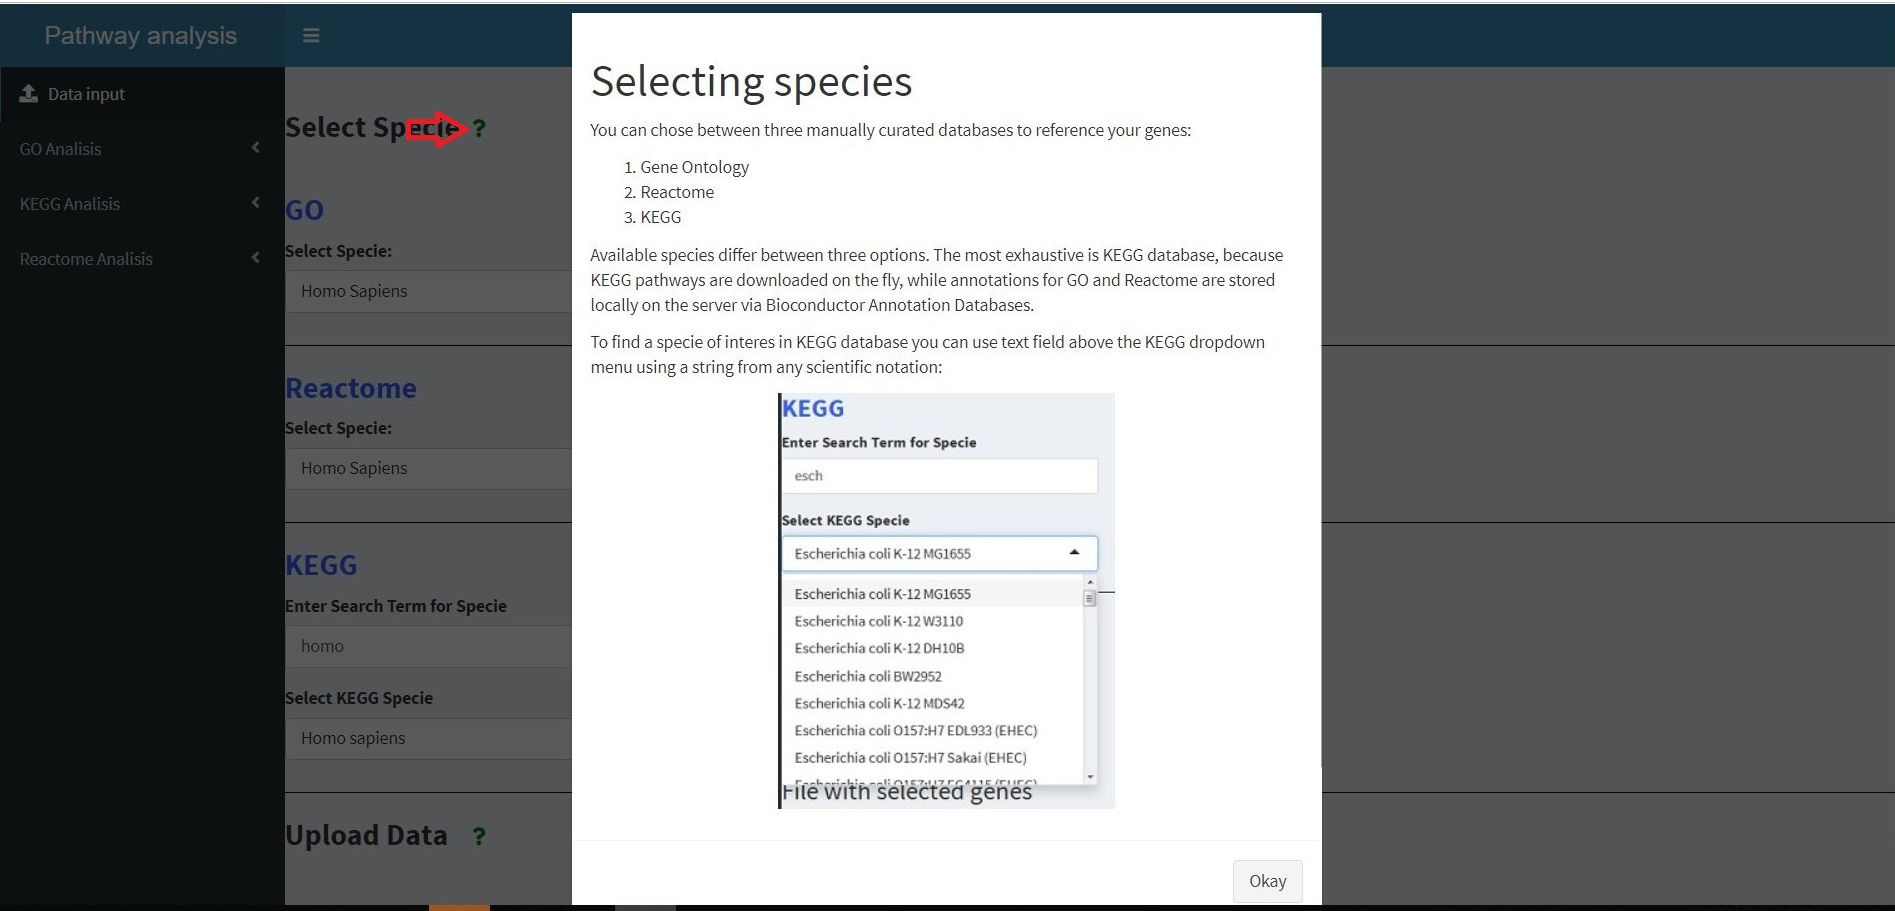
\includegraphics[width=0.9\textwidth]{Help_Specie.jpg} 
\caption{Ajuda per a l'elecció de l'espècie}
\end{figure}

\begin{figure}[H]
\centering
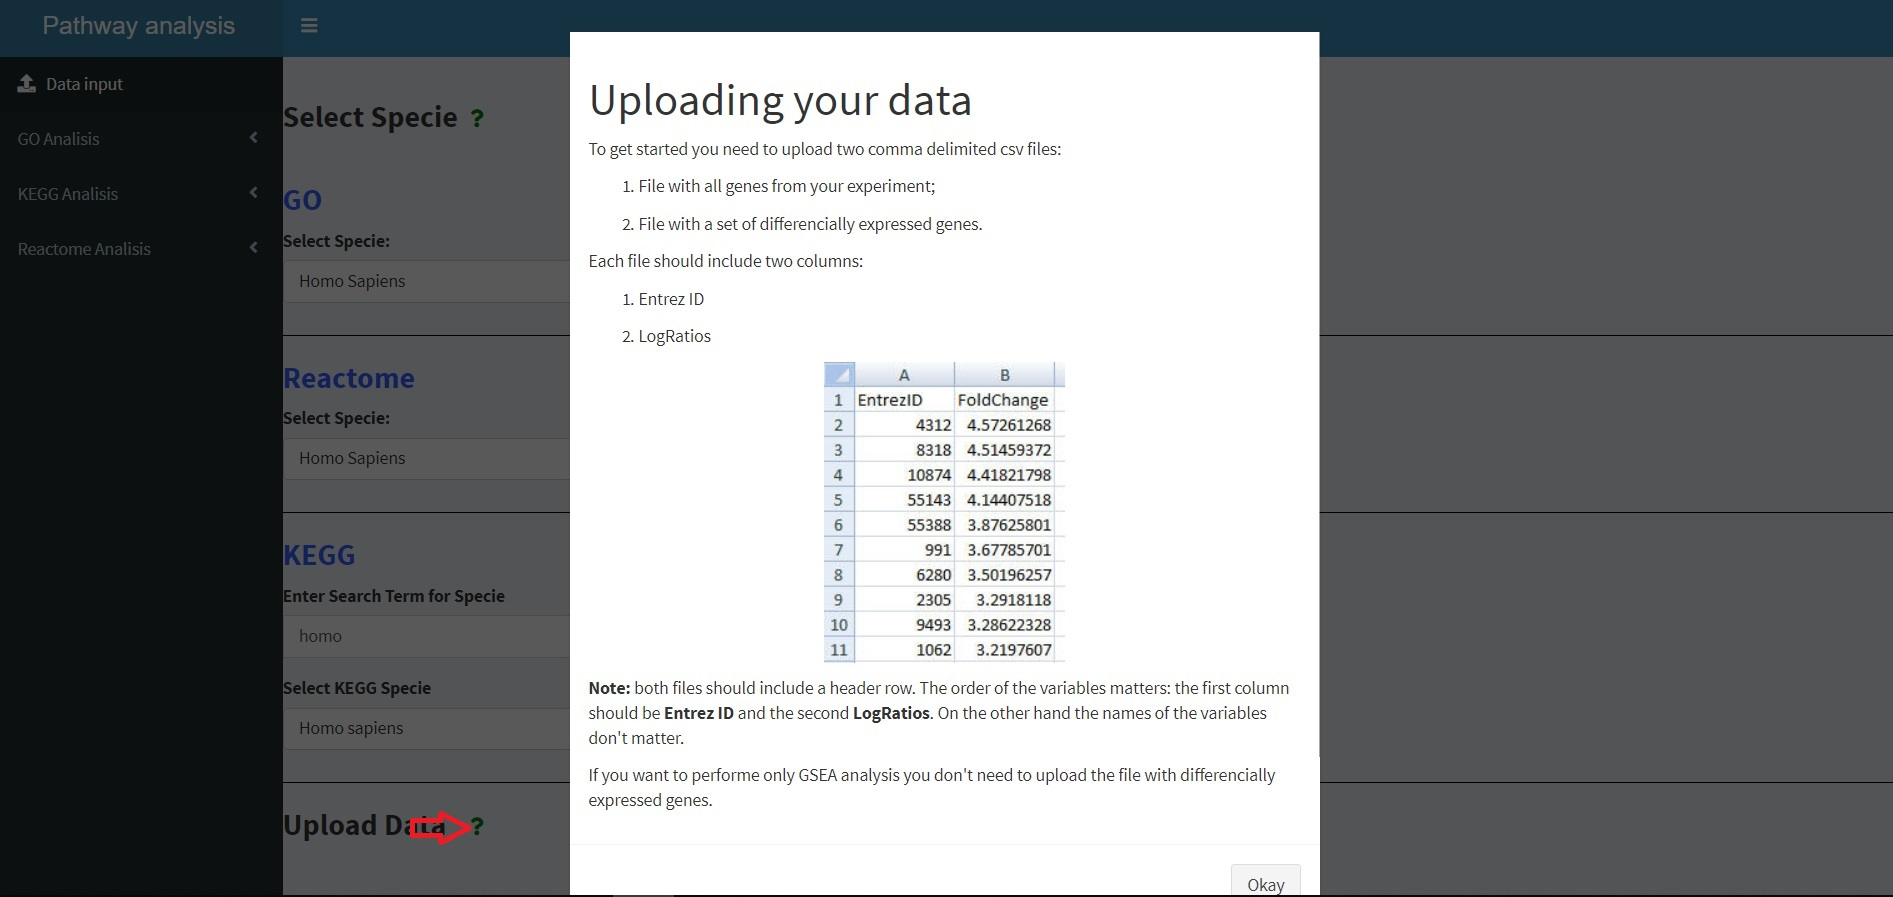
\includegraphics[width=0.9\textwidth]{Help_Upload_Data.jpg} 
\caption{Ajuda per pujar les dades}
\end{figure}

Les informacions per a l'apartat ORA són les següents:

\begin{figure}[H]
\centering
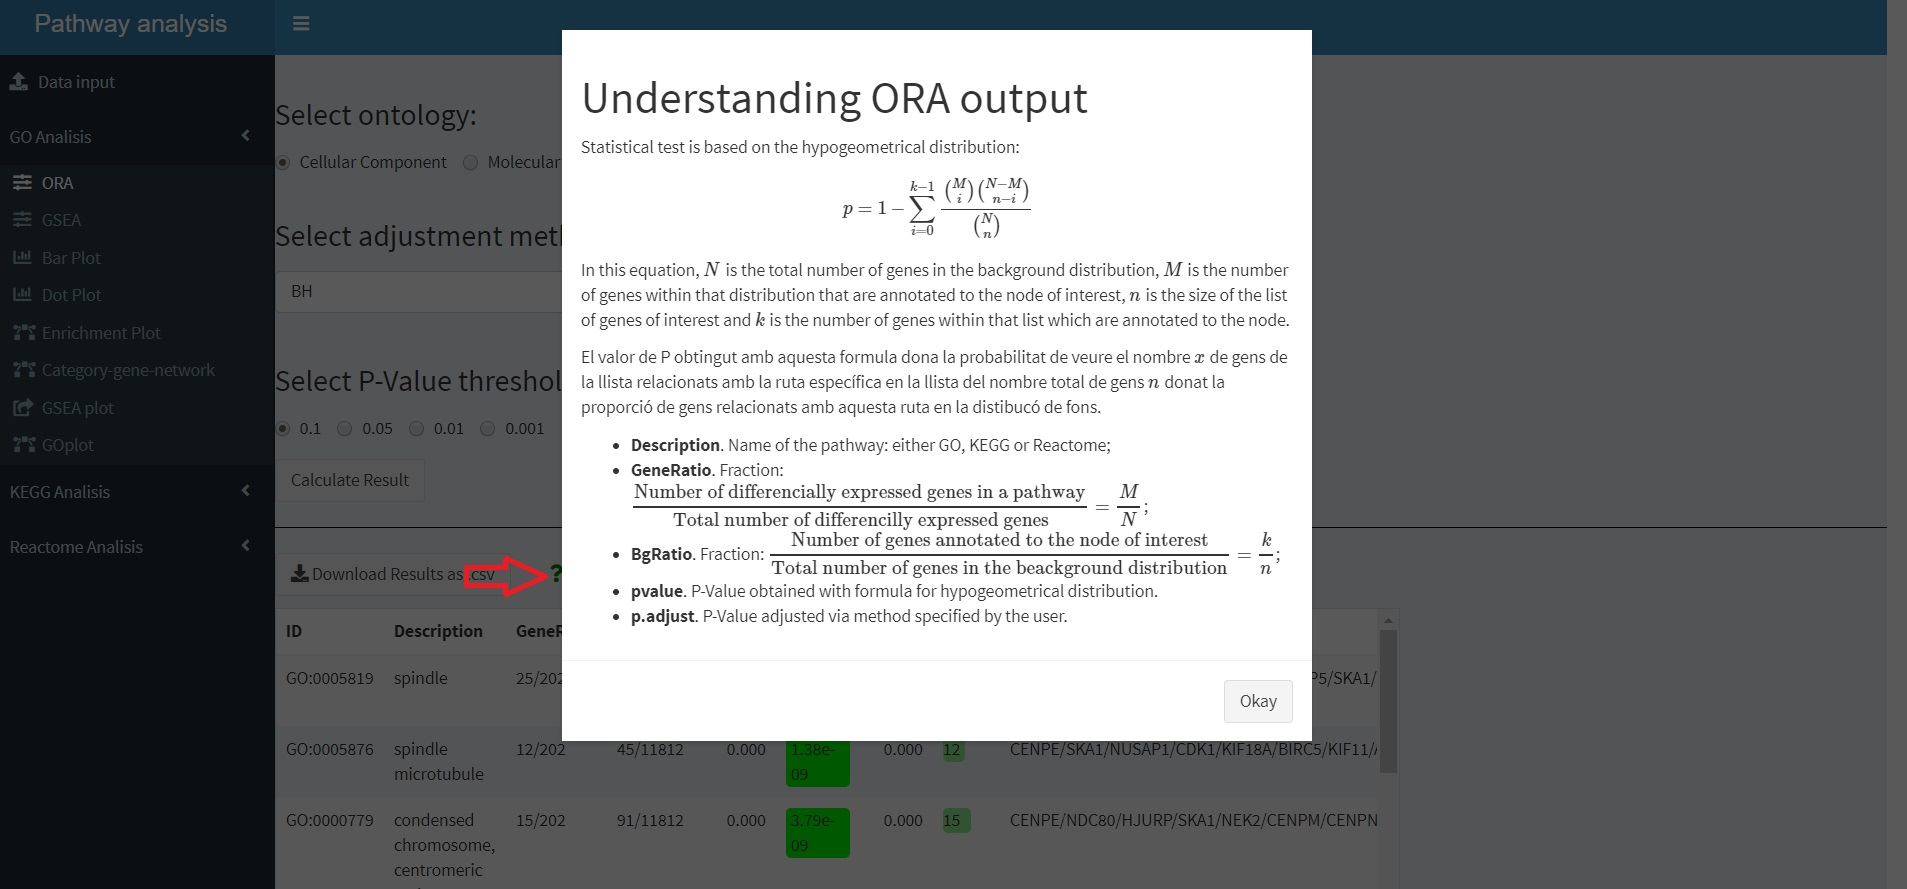
\includegraphics[width=0.9\textwidth]{Help_ORA_output.jpg} 
\caption{Infromació per la interpretació d'anàlisi ORA}
\end{figure}
Aquí cal destacar que les fòrmules, depenent de l'ordinador, no apareixen degudament en el RStudio Browser. Sí que apareixen bé quan l'aplicació s'obre via l’internet browser. L'usuari ha de tenir connexió amb internet perquè l'aplicació pugui descodificar la fòrmula via MathJax. Encara no he trobat la causa per la qual el Rstudio Browser en alguns ordinadors no visualitza bé les fòrmules. Pot ser un problema amb Java, que s'ha d'actualitzar? Ho estic investigant.

\begin{figure}[H]
\centering
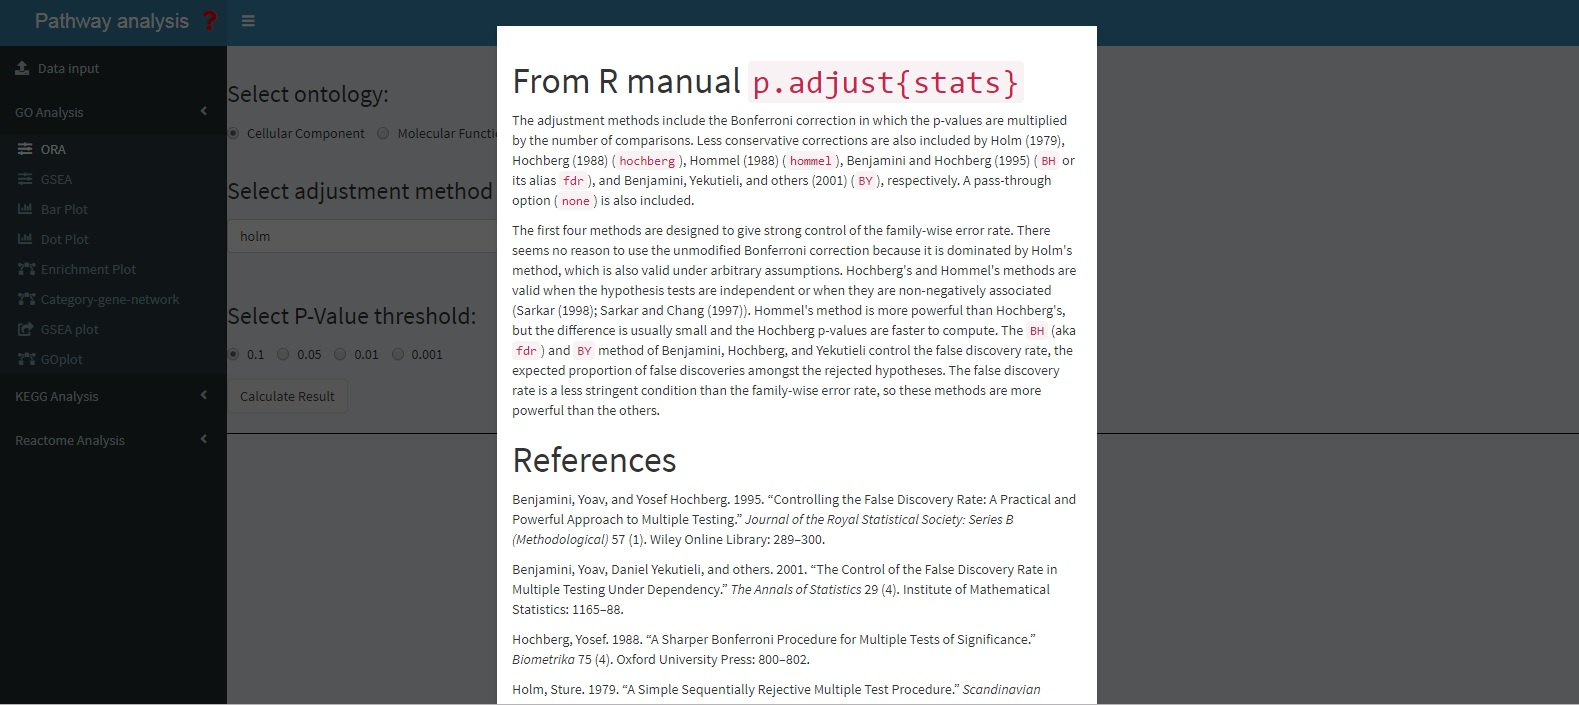
\includegraphics[width=0.9\textwidth]{Help_pAdjustMethod.jpg} 
\caption{L'ajuda per a la selecció del mètode d'ajustament}
\end{figure}


\begin{figure}[H]
\centering
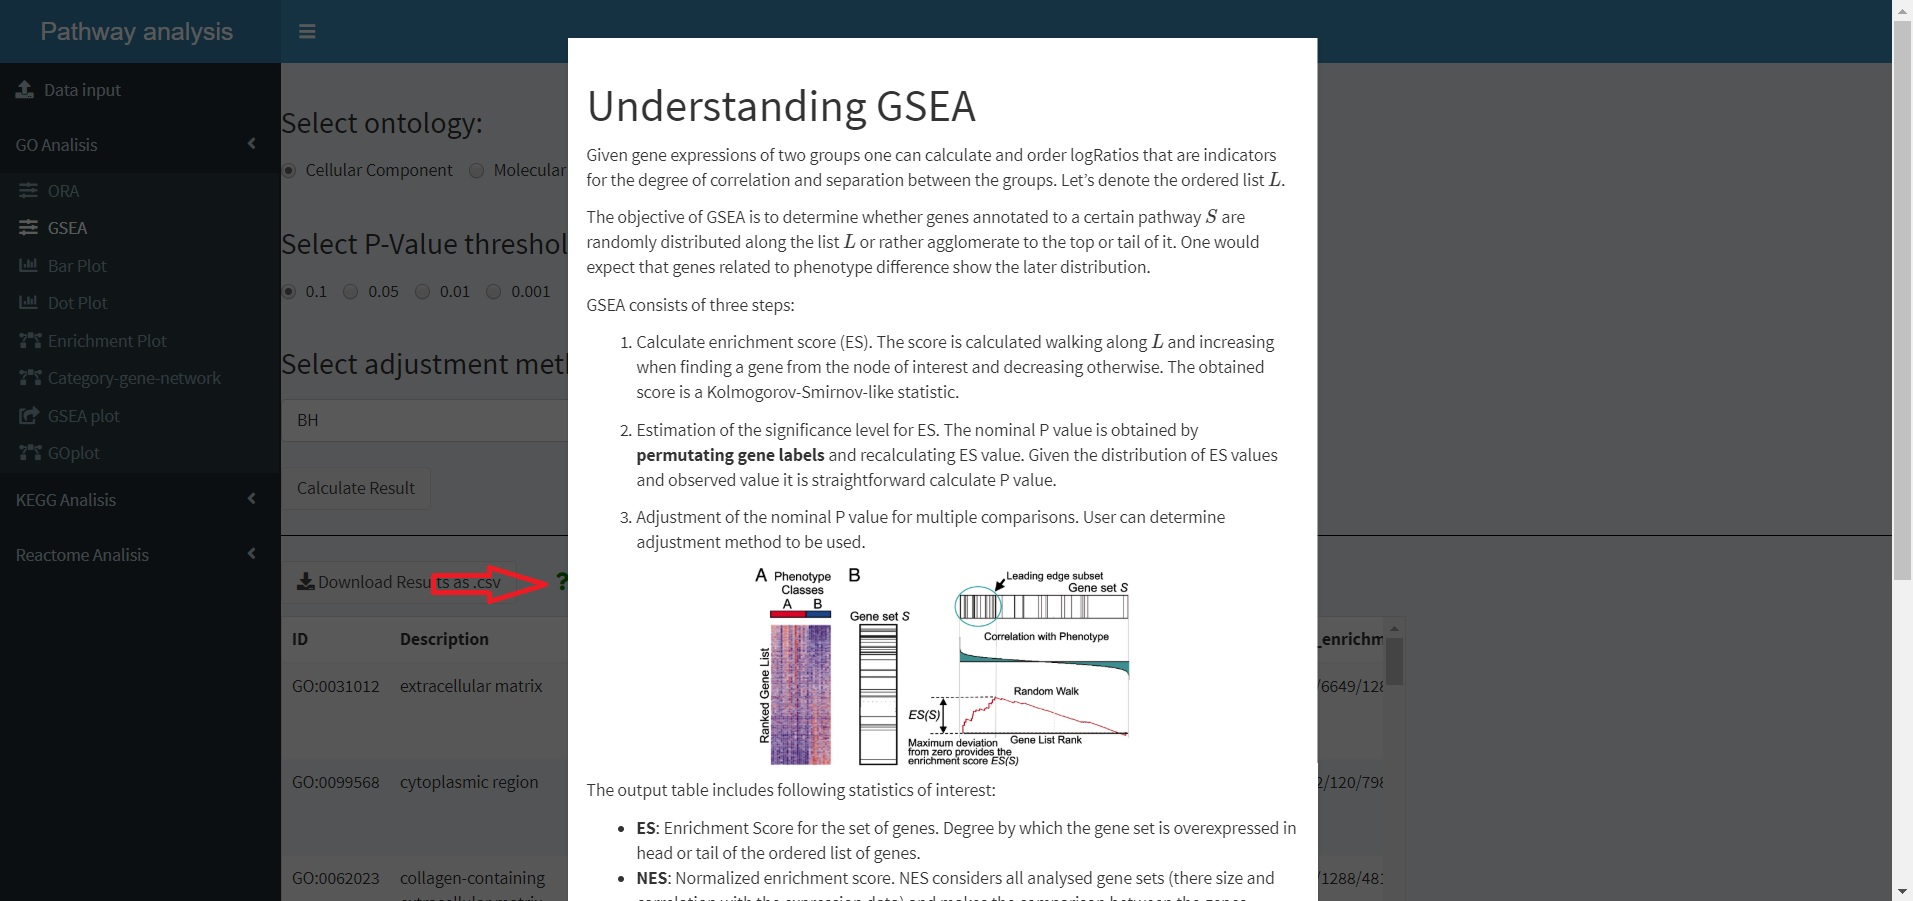
\includegraphics[width=0.9\textwidth]{Help_GSEA_output.jpg} 
\caption{Ajuda per la interpretació de GSEA}
\end{figure}

\subsection{Memoria}
Ja he començat a descriure els mètodes per a la memòria. El draft de la memòria l'adjunto juntament amb aquesta PAC. Clarament hi escriuré mès informació. Per ara, amb el temps disponible, m'he centrat en la descripció dels mètodes ORA i GSEA. A mès a mès encara no tinc disponible l'estructura predeterminda d'acord amb el pla docent. En les pròximes dues setmanes tindré temps suficient per acabar-la.

\section{Grau de compliment dels objectius.}
Mirem el calendari previst per a aquesta PAC
\begin{figure}[H]
\centering
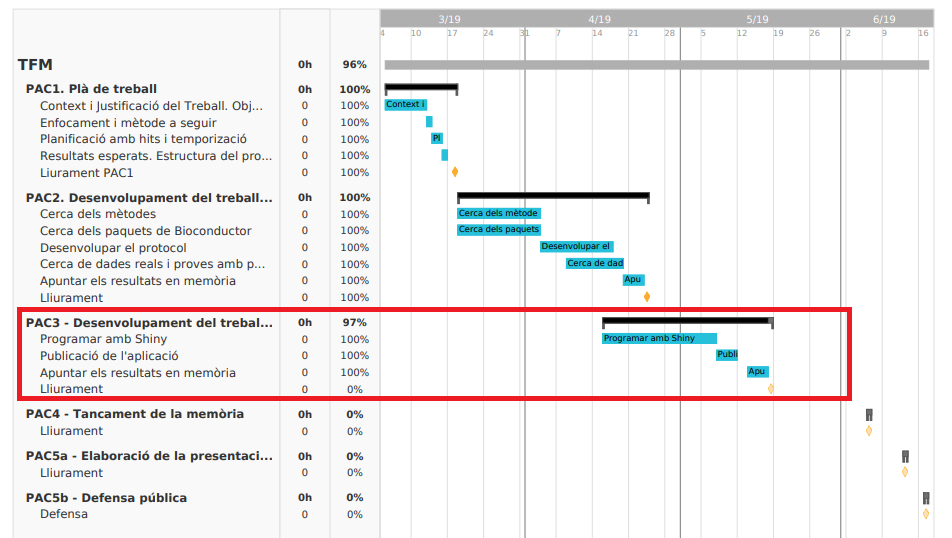
\includegraphics[width=0.9\textwidth]{Calender.png} 
\caption{Calender}
\end{figure}

Les activitats previstes eren:
\begin{enumerate}
\item \textbf{Programar amb Shiny};

Crec que he pogut millorar l'aplicació afegint el manual i les ajudes. Temporalment m'ha costat trobar i implementar les ajudes però finalment ho he aconseguit i estic content amb el resultat. Les millores en aquesta direcció (afegir més informació o més apartats al manual) ja no trigaran gaire, perquè ja sé com fer-ho.
\item \textbf{Publicació de l'aplicació}.

Com he explicat en el primer apartat, l’opció de publicació elegida és la via GitHub. Les altres opcions són també possibles però al mateix temps impliquen una feina fora del límit temporal previst pel TFM. 

\item \textbf{Apuntar els resultats en la memòria}.

Ja ho he començat a fer i estic segur que tenint l'aplicació acabada i rebent les instruccions determinades per part del professor acabaré la memòria ràpidament. 

\end{enumerate}

\section*{Biblilografia}
\addcontentsline{toc}{section}{Biblilografia}

\begingroup
\renewcommand{\section}[2]{}%
%\renewcommand{\chapter}[2]{}% for other classes
\bibliography{references}
\endgroup
\bibliographystyle{apalike}


\end{document}



